% !TeX root = ../../../main.tex
\subsection{Geometric Constraint Primitives}%
\label{sec:solution.impl.gcps}

Having overcome the language barrier between C++ and Julia, we can build our
\ac{GC} primitives on top of \texttt{CGAL.jl}.  Our implementation of the
\primitives{} is loosely inspired on tools like \texttt{tkz-euclide} and
Eukleides.  Both are based on Euclidean geometry, a constructive system where
the production of geometry can be done solely resorting to a straightedge and a
compass.  This makes programs described using these constructs easier to
understand and manually reproduce.

The following sections include a revisiting of our initially formulated example 
problems, described in \cref{sec:intro.examples}, and another set of primitives
that will be the driving force behind the case studies we go over later in
\cref{chap:eval}.

\subsubsection{Parallel lines}%
\label{sec:solution.impl.gcps.parallel}

Revisiting our earlier examples, we now showcase implementations for those
problems using our solution, accompanied by visualizations resorting to the
Khepri \ac{AD} tool.  \Cref{lst:solution.impl.gcps.parallel} shows a solution to
the ``parallel lines'' problem introduced in \cref{sec:intro.examples.parallel}.

\begin{listing}[htbp]
  \inputminted[highlightlines={4,6-7,16}]{julia}{jl/ex_parallel.jl}
  \caption[Parallel lines example using our solution]{
    Implementation of the parallel lines example illustrated in
    \cref{fig:intro.example.parallel} using Khepri alongside our solution.}%
  \label{lst:solution.impl.gcps.parallel}
\end{listing}

The first line highlighted in the program consists of the implementation of the
primitive construct.  The \texttt{parallel} function takes a line segment
\texttt{l}, the segment the resulting line is meant to be parallel to; and a
point \texttt{p} which the resulting line passes through.  We then build a new
line segment whose starting point is the given point \texttt{p}, and the end
point is the result of adding the difference between \texttt{l}'s endpoints to
\texttt{p}, obtained using \texttt{CGAL.jl}'s \texttt{to\_vector} function.

We then need to tell Khepri how to create objects our implementation can
understand by converting both the inputs and the resulting output.
\texttt{CGAL.jl} already contains a primitive shim of conversions between some
objects that facilitate this effort.\footnote{Ideally, the target \ac{AD} tool
would integrate our solution's constructs in a tighter more seamless fashion.}

Finally, we can use our primitive as seen highlighted in the listing,
reproducing the same result. \Cref{fig:solution.impl.gcps.parallel} illustrates
the formulated program's output in AutoCAD, one of the visualization tools
Khepri supports.

\begin{figure}[htbp]
  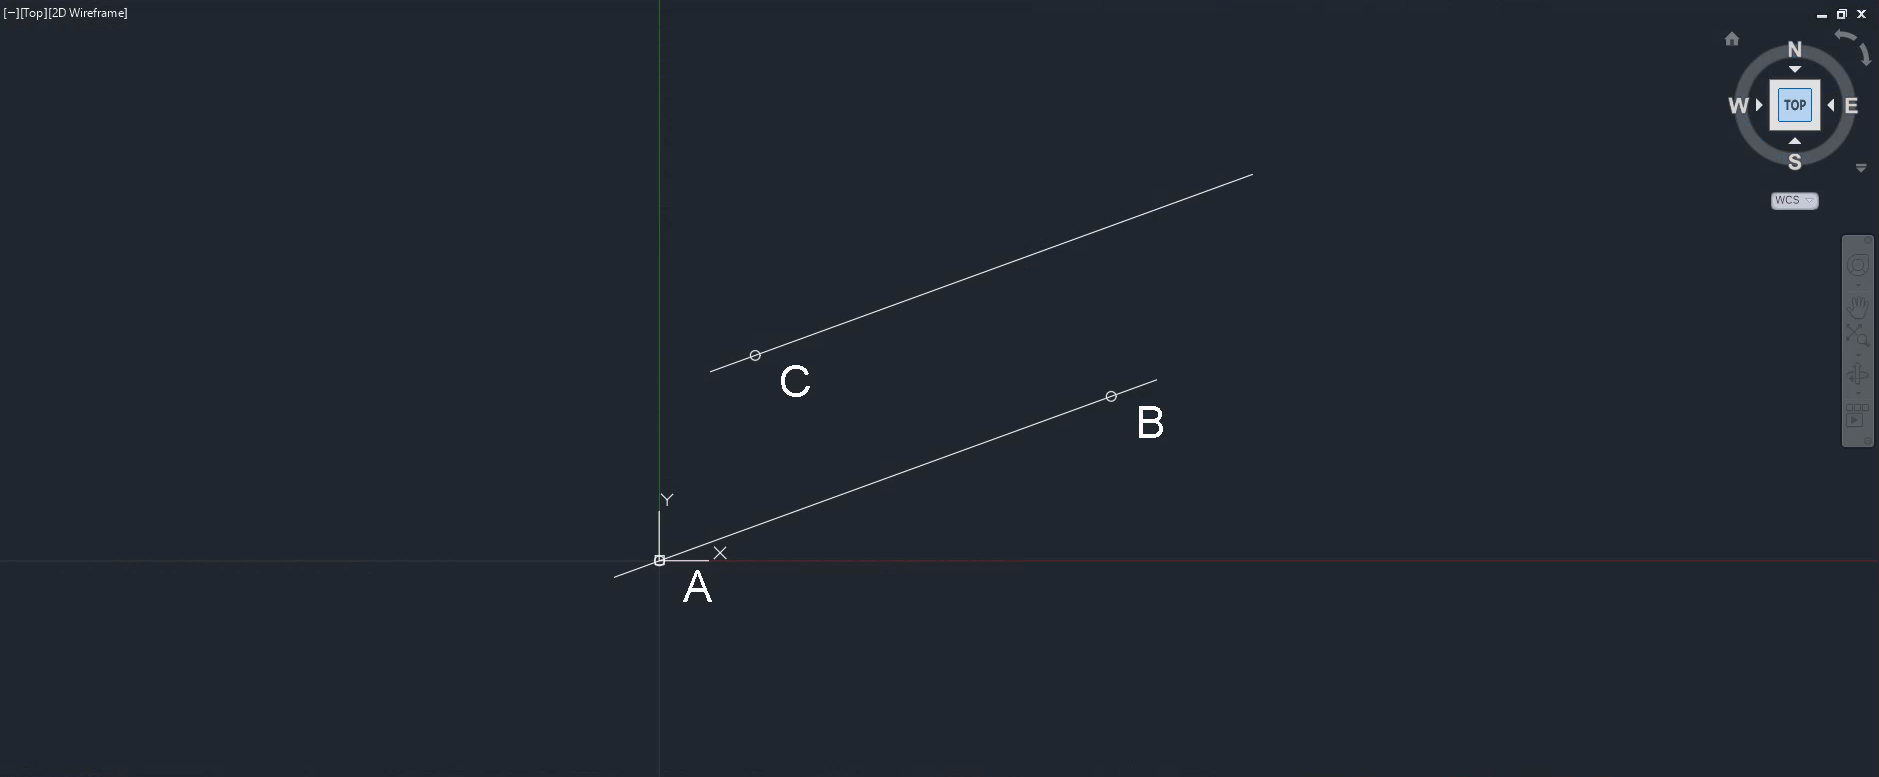
\includegraphics[width=\linewidth]{fig/autocad-parallel} 
  \caption[Parallel lines example using our solution]{
    Parallel lines example from \cref{sec:intro.examples.parallel} revisited
    using our solution's \texttt{parallel} primitive construct.  Output
    visualized in AutoCAD.}%
  \label{fig:solution.impl.gcps.parallel}
\end{figure}

\subsubsection{Circumcenter}%
\label{sec:solution.impl.gcps.circumcenter}

Regarding our circumcenter problem, introduced in
\cref{sec:intro.examples.circumcenter}, we initially solved it by intersecting
two of the three triangle sides' bisectors.  We can still approach the problem
that way, defining a \texttt{circumcenter} function similar to the one in
\cref{lst:solution.impl.gcps.circimpl}.

\begin{listing}[htbp]
  \begin{minted}{julia}
  circumcenter(a, b, c) = intersection(bisector(a, b), bisector(b, c)) 
  \end{minted}
  \caption[Initial circumcenter solution]{
    Initial implementation of the \texttt{circumcenter} function.}%
  \label{lst:solution.impl.gcps.circimpl}
\end{listing}

However, this is one occasion where this functionality is already present in
\ac{CGAL}.  This is a simple yet perfect demonstration of one of our approach's
benefits with regard to repurposing a comprehensive library with plenty of
functionality, allowing us near-direct reuse without re-implementing it.

\Cref{lst:solution.impl.gcps.circumcenter} illustrates a solution to the
``circumcenter'' problem using \ac{CGAL}'s \texttt{circumcenter} function.  The
program's output can be seen in \cref{fig:solution.impl.gcps.circumcenter}.

\begin{listing}[htbp]
  \inputminted[highlightlines={2,4-5,17}]{julia}{jl/ex_circumcenter.jl}
  \caption[Circumcenter example using our solution]{
    Implementation of the circumcenter example illustrated in
    \cref{fig:intro.example.circumcenter} using Khepri alongside our solution.}%
  \label{lst:solution.impl.gcps.circumcenter}
\end{listing}

\begin{figure}[htbp]
  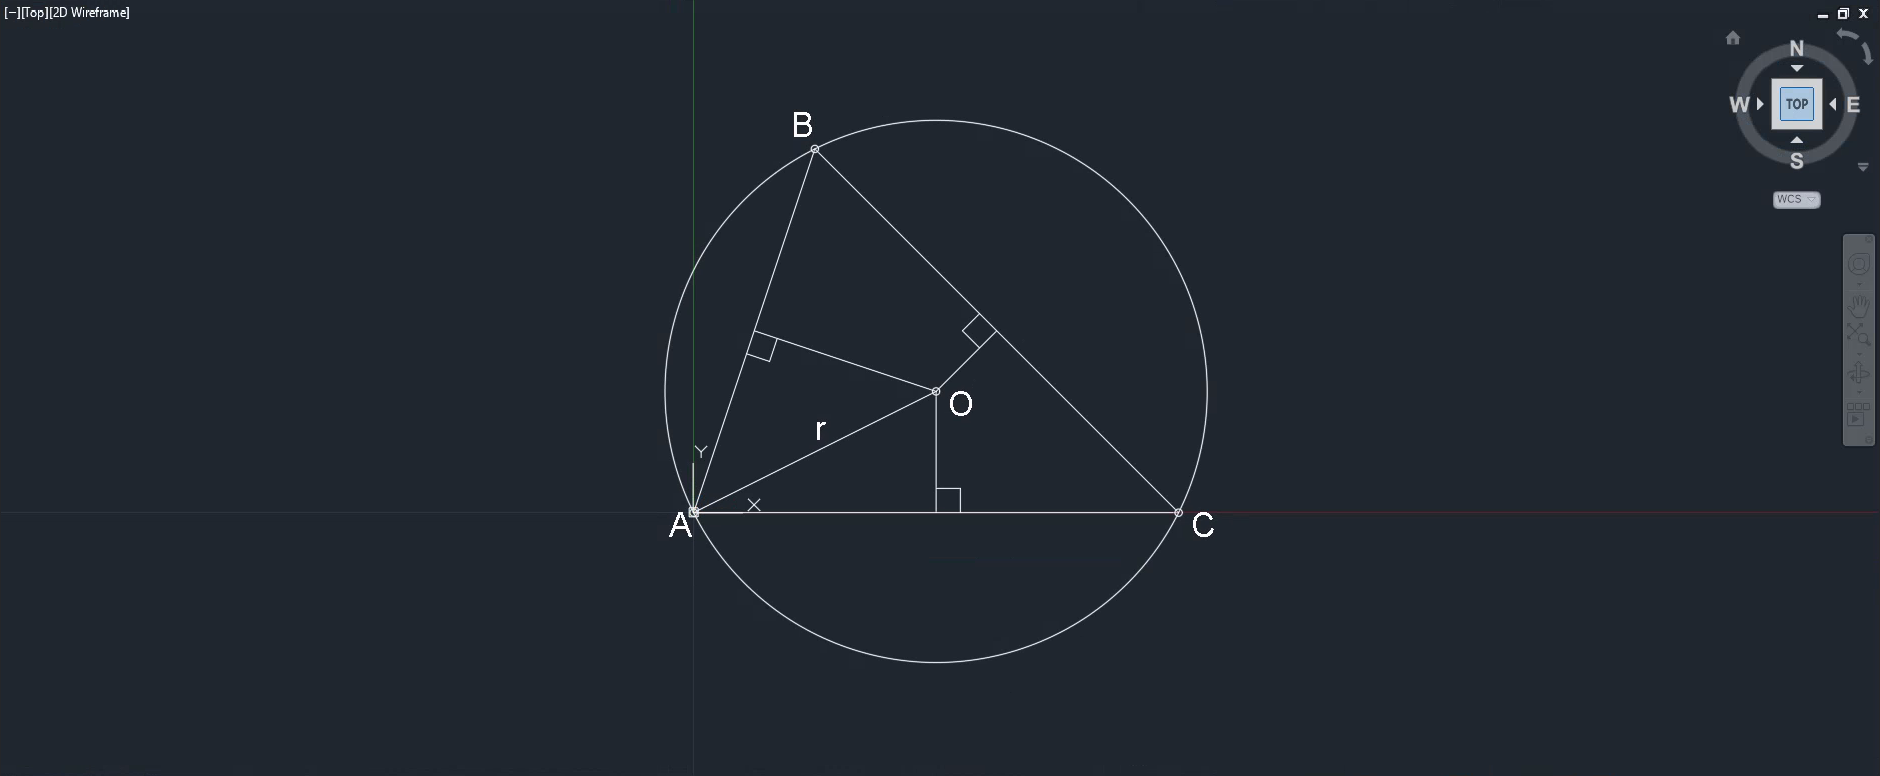
\includegraphics[width=\linewidth]{fig/autocad-circumcenter} 
  \caption[Circumcenter example using our solution]{
    Circumcenter example revisited using our solution's \texttt{circumcenter}
    primitive construct.  Output visualized in AutoCAD.}%
    \label{fig:solution.impl.gcps.circumcenter}
\end{figure}

\subsubsection{Circle tangent to a line}%
\label{sec:solution.impl.gcps.tangcirc2line}

Moving on to a set of problems that cannot as directly be solved by \ac{CGAL} is
that of tangencies.  Generally speaking, there are specific constructs available
in \ac{CGAL} that solve these problems.  However, we can once again repurpose
the ones we have and build on top of them.

This problem involves computing a circle that is tangent to an already existing
line.  Given the circle's center \texttt{o} and the line \texttt{l} we want the
circle to be tangent to, the tangent circle is such that its radius is the
minimal distance between its center point \texttt{o} and the line \texttt{l}.
The implementation of the problem's solution can be seen in
\cref{lst:solution.impl.gcps.tangcircle2line}.

\begin{listing}[htb]
  \begin{minted}{julia}
  tangent_circle(o::Point2, l::Line2) = Circle2(o, squared_distance(o, l))
  \end{minted}
  \caption[Circle tangent to a line]{
    Implementation of the ``Circle tangent to a line'' problem.}%
  \label{lst:solution.impl.gcps.tangcircle2line}
\end{listing}

Notice this solution considers we are working with infinite lines, not
necessarily line \textit{segments} in general.  Were we to apply the same simple
approach to a line segment, the circle would end up tangent to the line segment
as well.  However, the resulting circle could be tangent to one of the segment's
endpoints instead of tangent to a point along the segment.  In some cases, the
latter behavior may be preferred, for which adjustments to the solution must be
made, such as indicating that there is no solution for the given center point.

We did not implement such a scenario regarding line segments, because much like
the other primitives, it was created to quench a specific use case's thirst.  A
potential solution to that specific problem could be obtained reusing the
\texttt{tangent\_circle} function, however.  We would then need to verify if the
circle would fall somewhere between the segment's endpoints.  Otherwise, there
would not be a solution available.

\subsubsection{Tangent circles}%
\label{sec:solution.impl.gcps.tangentcircles}

Another instance of tangency is that of two circles tangent to each other.  This
proves to be a relatively more complex problem due to how the circles may be
positioned.

Given two circles \texttt{c\textsubscript{1}} and \texttt{c\textsubscript{2}},
and a vector \texttt{v} used to indicate the point of tangency on
\texttt{c\textsubscript{1}}, we draw a circle centered on said point with the
same radius as \texttt{c\textsubscript{2}} and intersect it with a ray
\texttt{r'} originating from the former circle's center, giving us a point
\texttt{f}.  This ray may be directed in one of two ways, determining if the
resulting circle contains both circles or not.  We then compute the bisector
\texttt{b} between \texttt{f} and \texttt{c\textsubscript{2}}.  We test if we
are in a situation where the resulting circle would instead turn out to be a
line.  If that is the case, we produce an error.  Otherwise, we construct the
tangent circle.

\Cref{lst:solution.impl.gcps.tangentcircles} contains the solution to the
problem, assisted by our own definition of the intersection function between a
circle and a ray, listed in \cref{lst:solution.impl.gcps.circrayint}.

\begin{listing}[htb]
  \inputminted[firstline=11]{julia}{jl/tangent_circles.jl}
  \caption[Tangent circles]{
    Implementation of the ``Tangent circles'' problem.}%
  \label{lst:solution.impl.gcps.tangentcircles}
\end{listing}

\begin{listing}
  \inputminted[lastline=9]{julia}{jl/tangent_circles.jl}
  \caption[Circle-Ray intersection]{
    Implementation of the intersection between a circle and a ray.}%
  \label{lst:solution.impl.gcps.circrayint}
\end{listing}

\subsubsection{Tangent lines between circles}%
\label{sec:solution.impl.gcps.tanglines2circles}

Another problem that surfaced in a case study earlier illustrated in
\cref{fig:intro.chair} is that of computing tangent lines between two circles.
It is a slightly more complex problem for which there is no obvious solution.
Fortunately, a constructive solution to this problem already
exists\footnote{\url{https://en.wikipedia.org/wiki/Tangent_lines_to_circles\#Synthetic_geometry}},
an approach our implementation is based on.

This problem's complexity lead us to break it into two different problems.
First, we must determine the lines tangent to a circle that pass through a given
point (\cref{lst:solution.impl.gcps.tanglines2circles}).  Then, repurposing the
solution to that problem, we solve the overarching problem of determining the
lines tangent between circles (\cref{lst:solution.impl.gcps.tanglines2circle}).
This is another example of how we can compose a smaller set of our primitives to
solve a larger problem.

\begin{listing}[htbp]
  \inputminted[firstline=2,lastline=16]{julia}{jl/circ_tangent_lines.jl}
  \caption[Tangent lines to a circle]{
    Implementation of the ``Tangent lines to a circle'' sub-problem.}%
  \label{lst:solution.impl.gcps.tanglines2circles}
\end{listing}

\begin{listing}[htbp]
  \caption[Tangent lines between circles]{
    Implementation of the ``Tangent lines between circles'' problem by way of
    composition with the solution of ``Tangent lines to a circle''.}%
  \label{lst:solution.impl.gcps.tanglines2circle}
  \inputminted[firstline=18,lastline=59]{julia}{jl/circ_tangent_lines.jl}
\end{listing}

Our implementation returns the results in a deterministic way, facilitating
result choice.  The line segments are oriented from \texttt{c\textsubscript{1}}
to \texttt{c\textsubscript{2}}, with the internal tangents surrounded by the
external tangents, sorted in a counterclockwise orientation.
